\documentclass[border=0.125cm]{standalone}
\usepackage{tikz}
\usetikzlibrary{matrix,positioning,calc, automata}
\begin{document}
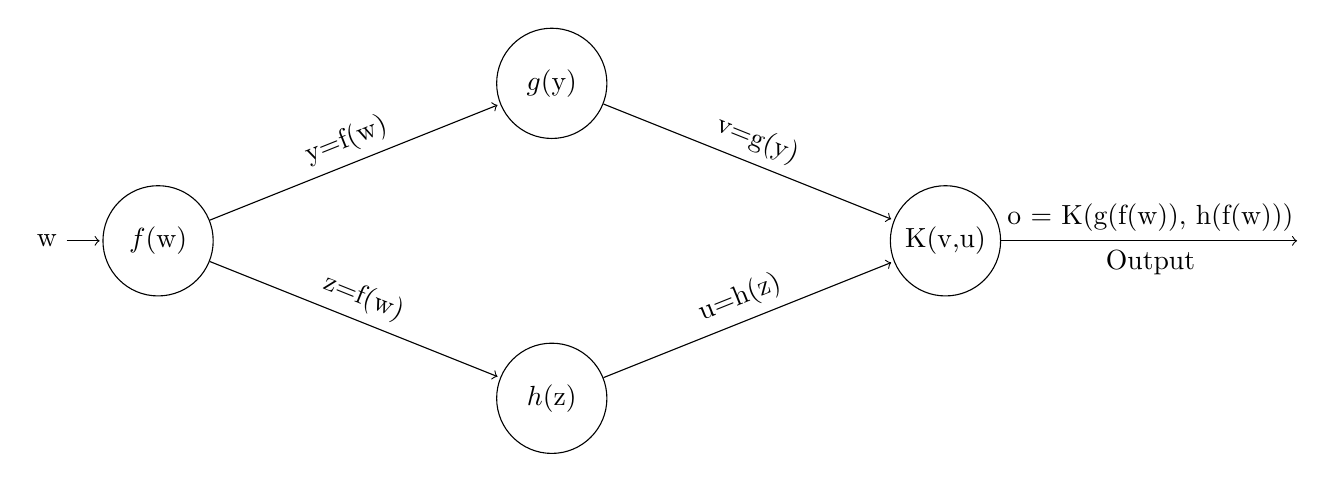
\begin{tikzpicture}[shorten >=1pt,on grid]
  
  \node[state,initial, initial text=w,minimum size=1.4cm]   (q0){$f(\textup{w})$};
  \node[state,minimum size=1.4cm] (q1) at (5,2) {$g(\textup{y})$};
  \node[state,minimum size=1.4cm] (q2) at (10,0) {$\textup{K}(\textup{v,u})$};
  \node[state,minimum size=1.4cm] (q3) at (5,-2) {$h(\textup{z})$};
  \path[->] (q0) edge                node [above,sloped] {y=f(w)} (q1)
            (q1) edge                node [above,sloped] {v=g(y)} (q2)
            (q0) edge                node [above,sloped] {z=f(w)} (q3)
            (q3) edge                node [above,sloped] {u=h(z)} (q2);
  \draw[->](q2)--node[below]{Output}node[above]{o = K(g(f(w)), h(f(w)))}(14.5,0);
  \end{tikzpicture}
\end{document}